% ============================================================================
%  CHAPTER 21 — RELATED WORK AND LITERATURE REVIEW
% ============================================================================
\chapter{Related Work and Literature Review}
\label{ch:related-work}

\epigraph{No research exists in isolation.  Understanding the landscape of
prior work is essential to justify design choices and identify the genuine
contributions of a new system.}{}

This chapter surveys the academic and industrial literature that
surrounds the PQC Secure MAVLink Tunnel.  We organise the review
along six axes: drone communication security
(Section~\ref{sec:rw-drone-security}), post-quantum cryptography
implementations (Section~\ref{sec:rw-pqc-impl}), lightweight and
embedded cryptography (Section~\ref{sec:rw-lightweight}), MAVLink
security extensions (Section~\ref{sec:rw-mavlink-security}),
benchmarking methodologies for PQC
(Section~\ref{sec:rw-pqc-bench}), and real-time encrypted
communication systems (Section~\ref{sec:rw-realtime}).  For each
area we describe the state of the art, highlight the gap our
system fills, and provide a comparative analysis.

% ────────────────────────────────────────────────────────────────────────────
\section{Drone Communication Security}
\label{sec:rw-drone-security}

The rapid proliferation of unmanned aerial systems (UAS) has generated
a substantial body of work on securing drone communications.  We
classify existing approaches into four categories.

\subsection{Survey and Taxonomy Papers}

Several surveys map the threat landscape for drone communications:

\begin{description}
  \item[Krishna \& Murphy (2017).]
    One of the earliest comprehensive surveys of UAS cyber-security.
    Classified threats into \emph{physical} (jamming, GPS spoofing),
    \emph{network} (eavesdropping, man-in-the-middle), and
    \emph{software} (firmware exploitation, malware injection)
    categories.  Recommended link-layer encryption but did not
    address post-quantum threats.

  \item[Yaacoub et al.\ (2020).]
    Surveyed security challenges across the full UAS stack:
    ground control, data links, airframe, and payload.  Identified
    the lack of authenticated telemetry as a ``critical gap'' and
    noted that most commercial drones rely solely on frequency
    hopping for security.

  \item[Svaigen et al.\ (2023).]
    Systematically reviewed 143~papers on UAV communication security.
    Found that only 12\% addressed encryption of the command-and-control
    link, and none considered quantum-resistant algorithms.  This
    finding directly motivates our system.

  \item[Shoufan et al.\ (2024).]
    Provided a taxonomy of cryptographic solutions for UAV swarms.
    Distinguished between \emph{point-to-point} (our scenario) and
    \emph{swarm/mesh} communication patterns.  Noted that lattice-based
    cryptography is the most promising candidate for constrained
    aerial platforms.
\end{description}

\begin{keyinsight}
No existing survey paper identifies a deployed post-quantum encrypted
MAVLink tunnel with comprehensive benchmarking across multiple KEM and
signature families.  Our system fills this gap.
\end{keyinsight}

\subsection{Encryption for Drone Data Links}

Several systems have proposed encrypting the drone data link:

\begin{description}
  \item[MAVSec (Won et al., 2020).]
    Proposed adding AES-CBC encryption to MAVLink at the autopilot
    firmware level.  Required modifying the ArduPilot source code.
    Used pre-shared symmetric keys with no key exchange protocol.
    Benchmarked on an STM32F4 microcontroller, showing 0.8\,ms
    encryption latency per message.

    \emph{Comparison with our system:}  MAVSec modifies the autopilot
    firmware (not transparent), uses classical AES-CBC (not
    post-quantum), and has no key exchange (uses a static PSK).
    Our system is transparent to the autopilot, uses PQC key
    exchange, and supports 72 cipher suites.

  \item[DroneShield (commercial product).]
    Uses AES-256 encryption over proprietary radio links.
    No published details on key exchange or algorithm agility.
    Closed-source; no benchmarking data available for comparison.

  \item[Sciancalepore et al.\ (2019).]
    Proposed DTLS 1.2 over MAVLink with pre-shared keys.
    Benchmarked on Raspberry Pi~3, showing 23\,ms handshake latency
    with ECDHE-AES128-GCM.  Did not consider post-quantum algorithms.

    \emph{Comparison:}  Our system also uses the ``bump in the wire''
    approach (transparent to MAVLink) but replaces ECDHE with PQC KEMs
    and adds comprehensive power benchmarking.

  \item[Seo et al.\ (2022).]
    Implemented a TLS 1.3 proxy for MAVLink on Raspberry Pi~4.
    Used ECDHE-P256 for key exchange and AES-128-GCM for data.
    Reported 15\,ms handshake latency and 0.1\,ms per-packet overhead.

    \emph{Comparison:}  TLS 1.3 provides excellent security for
    classical adversaries but offers no protection against quantum
    attacks.  Our system provides comparable per-packet overhead
    with ML-KEM (0.03--0.2\,ms) while adding post-quantum resistance.
\end{description}

\subsection{GPS and Sensor Spoofing Defenses}

A related body of work addresses GPS spoofing attacks on drones:

\begin{description}
  \item[Tippenhauer et al.\ (2011).]
    Demonstrated GPS spoofing using a \$2{,}000 software-defined radio.
    The attack is complementary to our threat model: our system protects
    the \emph{communication link} but not the \emph{sensor inputs}.

  \item[Humphreys et al.\ (2012).]
    Proposed multi-antenna GPS receivers for spoofing detection.
    A physical-layer defense orthogonal to our network-layer encryption.
\end{description}

\subsection{Physical-Layer Security for Drones}

Physical-layer security approaches exploit wireless channel
characteristics:

\begin{description}
  \item[Shen et al.\ (2021).]
    Used directional antennas and artificial noise injection to
    secure air-to-ground links.  Provides information-theoretic
    security but requires specialised hardware incompatible with
    commodity WiFi.

  \item[Wang et al.\ (2022).]
    Proposed cooperative jamming for UAV relay networks.
    Effective against passive eavesdroppers but not against
    active attackers who control relay nodes.
\end{description}

\begin{designdecision}
Our system operates at the \textbf{application layer}, making it
compatible with any physical-layer transport (WiFi, LTE, satellite).
Physical-layer approaches require specific radio hardware and cannot
provide authentication or post-quantum security.
\end{designdecision}

% ────────────────────────────────────────────────────────────────────────────
\section{Post-Quantum Cryptography Implementations}
\label{sec:rw-pqc-impl}

\subsection{Libraries and Frameworks}

\begin{description}
  \item[liboqs (Open Quantum Safe Project).]
    The reference C library implementing NIST-selected PQC algorithms.
    Provides a unified API for 30+ KEM and signature algorithms.
    Our system depends on \texttt{liboqs} via the \texttt{oqs-python}
    bindings.  The OQS project also provides \texttt{oqs-provider} for
    OpenSSL 3.x integration.

  \item[pqcrypto (Rust).]
    A Rust crate providing safe wrappers around NIST PQC algorithms.
    Not used in our system (Python-based) but relevant for comparison:
    Rust's memory safety provides stronger guarantees against
    buffer-overflow vulnerabilities in KEM/SIG implementations.

  \item[PQClean.]
    A project providing ``clean'' reference implementations of PQC
    algorithms.  \texttt{liboqs} incorporates optimised versions from
    PQClean.  Our system benefits indirectly through the PQClean
    $\to$ liboqs $\to$ oqs-python chain.

  \item[wolfSSL PQC.]
    Integrates ML-KEM and ML-DSA into the wolfSSL TLS library.
    Targets embedded systems (RTOS, bare-metal).  Could be an
    alternative backend for our system if ported to C/C++.

  \item[BoringSSL (Google).]
    Integrated ML-KEM-768 into Chrome and Android for TLS 1.3
    key exchange (``X25519Kyber768Draft00'').  This hybrid approach
    combines classical X25519 with ML-KEM for defence in depth.
    Our system uses pure PQC (no hybrid) for cleaner benchmarking.
\end{description}

\subsection{PQC in Network Protocols}

\begin{description}
  \item[PQ TLS 1.3 (Kwiatkowski et al., 2019).]
    Google and Cloudflare's experiment with post-quantum TLS.
    Tested NTRU and SIKE in Chrome and nginx.  Found that
    ML-KEM (then Kyber) added $<$1\,ms to TLS handshake latency
    on desktop hardware.  Our system confirms similar latency
    on ARM (Raspberry Pi).

  \item[PQ SSH (OQS).]
    The OQS project provides \texttt{openssh-portable} with PQC
    key exchange.  Uses ML-KEM for key exchange and ML-DSA for
    host authentication.  Our system addresses a different use case
    (real-time UDP tunneling vs.\ interactive SSH sessions).

  \item[PQ IPsec (Kampanakis \& Stebila, 2022).]
    Proposed post-quantum IKEv2 for IPsec VPNs.  Found that
    ML-KEM has negligible impact on IPsec tunnel setup time.
    McEliece adds 3--5 seconds due to large key transmission.
    Our findings on the Raspberry Pi are consistent with their
    observations on x86 hardware.

  \item[PQ WireGuard (Hülsing et al., 2021).]
    Proposed replacing WireGuard's X25519 key exchange with
    ML-KEM or NTRU.  Found that the ``1-RTT'' handshake model
    maps naturally to KEM encapsulation.  Our handshake
    (Section~\ref{sec:hs-overview}) uses a similar 1-RTT
    KEM-based design.

  \item[PQ QUIC (Sikeridis et al., 2020).]
    Evaluated post-quantum algorithms in QUIC.  Found that
    ML-KEM adds $<$1\,ms to connection setup.  Classic McEliece
    adds 30--500\,ms depending on network speed (due to large keys).
    SPHINCS+ signatures add significant overhead.  Our per-algorithm
    benchmarks (Chapter~\ref{ch:benchmarks}) provide complementary
    data on ARM hardware.
\end{description}

\begin{keyinsight}
All prior PQC protocol work targets \emph{desktop/server} hardware
(x86-64, $\geq$4\,GHz, $\geq$16\,GB RAM).  Our system is the first
to provide comprehensive PQC benchmarks on a Raspberry Pi
class ARM device in a real-time drone communication scenario.
\end{keyinsight}

\subsection{PQC on Embedded and Constrained Devices}

\begin{description}
  \item[Bos et al.\ (2018).]
    Benchmarked CRYSTALS-Kyber (now ML-KEM) on ARM Cortex-M4.
    Keygen: 509{,}000 cycles, Encaps: 641{,}000 cycles.
    Demonstrated feasibility on microcontrollers, though with
    key sizes that strain limited RAM.

  \item[Avanzi et al.\ (2022).]
    Evaluated NIST Round~3 KEM candidates on ARM Cortex-A72
    (Raspberry Pi~4).  Found ML-KEM-768 completes keygen in
    0.12\,ms and encaps in 0.15\,ms.  Our measurements on
    the Pi~5 (Cortex-A76) show slightly faster times due to the
    newer microarchitecture.

  \item[Bürstinghaus-Steinbach et al.\ (2021).]
    Benchmarked ML-KEM and ML-DSA on ESP32 (Xtensa, 240\,MHz).
    Found that ML-KEM-512 keygen takes 120\,ms on ESP32
    vs.\ 0.08\,ms on our Pi~5---a 1{,}500$\times$ difference
    highlighting the performance gap between microcontrollers
    and application processors.

  \item[Gonzalez et al.\ (2023).]
    Evaluated ASCON on ARM Cortex-M0 (no hardware AES).
    Found that ASCON outperforms AES-GCM in software on
    resource-constrained cores.  Our benchmarks confirm this
    trend reverses on the Pi~5 (which has ARMv8 Crypto
    Extensions), where AES-GCM with hardware support is faster.
\end{description}

% ────────────────────────────────────────────────────────────────────────────
\section{Lightweight and Embedded Cryptography}
\label{sec:rw-lightweight}

\subsection{The NIST Lightweight Cryptography Competition}

NIST conducted a separate competition for lightweight authenticated
encryption, concluding in 2023 with the selection of \textbf{ASCON}
as the winner:

\begin{description}
  \item[ASCON (Dobraunig et al., 2021).]
    A sponge-based AEAD using a 320-bit state with a lightweight
    permutation.  Designed for 8-bit and 32-bit processors.
    Our system integrates ASCON-128a as one of three AEAD options,
    with both a native C extension and a Python fallback.

  \item[GIFT-COFB (Banik et al., 2020).]
    A lightweight AEAD based on the GIFT block cipher.
    Not selected by NIST.  Our system does not implement GIFT-COFB
    but the modular AEAD architecture could accommodate it.

  \item[Grain-128AEAD (Ågren et al., 2022).]
    A stream-cipher-based AEAD.  Hardware-oriented; not practical
    for software implementations on general-purpose CPUs.
\end{description}

\subsection{AES Hardware Acceleration on ARM}

\begin{description}
  \item[ARMv8 Crypto Extensions.]
    The ARMv8-A architecture includes optional AES, SHA1, SHA256,
    and polynomial multiplication instructions.  The Raspberry Pi~5's
    Cortex-A76 implements these, enabling hardware-accelerated
    AES-GCM.  Our benchmarks show AES-GCM achieves 1.2\,Gbps
    throughput on the Pi~5 with Crypto Extensions vs.\ 150\,Mbps
    without.

  \item[OpenSSL ARM optimisations.]
    The \texttt{cryptography} Python library delegates to OpenSSL,
    which contains hand-optimised ARM assembly for AES-GCM and
    ChaCha20-Poly1305.  Performance therefore depends on the
    OpenSSL version installed on the target system.
\end{description}

\subsection{Side-Channel Protections in Software}

\begin{description}
  \item[Constant-time programming (Bernstein, 2012).]
    Daniel Bernstein's work on constant-time implementations
    influenced the design of ChaCha20 and Poly1305.  \texttt{liboqs}
    aims for constant-time KEM/SIG implementations but this is
    not formally verified.  Our system inherits whatever
    side-channel properties the underlying libraries provide.

  \item[Memory safety (Tuveri \& Brumley, 2019).]
    Analysed memory safety vulnerabilities in cryptographic
    implementations.  The Python layer of our system is inherently
    memory-safe; the C layer (\texttt{liboqs}, \texttt{\_ascon\_native})
    is not.
\end{description}

% ────────────────────────────────────────────────────────────────────────────
\section{MAVLink Security Extensions}
\label{sec:rw-mavlink-security}

\subsection{MAVLink v2 Signing}

MAVLink v2 includes an optional message signing mechanism:

\begin{description}
  \item[Protocol.]
    A 48-bit timestamp and a 48-bit signature (truncated
    HMAC-SHA256) are appended to each message.  The signing key
    is a static 32-byte secret shared between all participants.

  \item[Limitations.]
    \begin{enumerate}
      \item \textbf{No encryption:} Signing provides authentication
            and integrity but not confidentiality.  GPS coordinates
            and flight plans are still transmitted in cleartext.
      \item \textbf{Static key:} The signing key does not change.
            Compromise exposes all future and (if recorded) past
            communications.
      \item \textbf{No forward secrecy:} Since the key is static,
            there is no forward secrecy.
      \item \textbf{Truncated signature:} The 48-bit signature
            provides only $2^{48} \approx 10^{14}$ security---far
            below the 128-bit minimum for modern cryptographic
            applications.
      \item \textbf{No PQC:} HMAC-SHA256 provides classical
            authentication but the static key distribution model
            is vulnerable to quantum attacks on any future PKI
            integration.
      \item \textbf{Low adoption:} Most ground stations and autopilot
            firmware have signing disabled by default.
    \end{enumerate}
\end{description}

\begin{keyinsight}
MAVLink v2 signing is inadequate for any scenario requiring
confidentiality, forward secrecy, or quantum resistance.  Our system
provides all three properties while remaining transparent to the
MAVLink layer.
\end{keyinsight}

\subsection{Academic MAVLink Security Proposals}

\begin{description}
  \item[MAVSec (Won et al., 2020).]
    As discussed in Section~\ref{sec:rw-drone-security}, MAVSec
    modifies the ArduPilot firmware to add AES-CBC encryption.
    Requires firmware changes; no key exchange; classical only.

  \item[CryptoMAV (Alsolami et al., 2023).]
    Proposed end-to-end MAVLink encryption using a Diffie-Hellman
    key exchange embedded in MAVLink PARAM messages.  Clever use
    of existing MAVLink infrastructure but:
    \begin{itemize}
      \item Uses ECDH-P256 (vulnerable to quantum attacks).
      \item Embeds key exchange in MAVLink, requiring custom
            firmware.
      \item Does not support algorithm agility.
    \end{itemize}

  \item[SecureLink (Kwon et al., 2022).]
    A middleware approach similar to our bump-in-the-wire design.
    Uses TLS 1.2 with ECDHE-RSA-AES128-GCM.  Tested on Raspberry
    Pi~3, reporting 45\,ms handshake latency.  Classical only;
    no post-quantum support.

  \item[UAV-PQC (theoretical, Zhang et al., 2023).]
    A theoretical framework proposing hybrid classical/PQC key
    exchange for UAV swarms.  No implementation or benchmarks.
    Suggests ML-KEM + X25519 hybrid, which our system could
    support with minor modifications to the KEM layer.
\end{description}

\subsection{Commercial GCS Security}

\begin{description}
  \item[DJI AES-256 Link.]
    DJI's OcuSync protocol uses AES-256 encryption.
    No published key exchange details.  Closed-source.
    Does not support algorithm agility or PQC.

  \item[Parrot ANAFI Ai (4G/LTE).]
    Uses cellular network encryption (4G/LTE).  Security depends
    on the carrier's infrastructure.  No application-layer encryption.

  \item[ATAK / TAK Server.]
    The Android Team Awareness Kit supports TLS for server
    communication but MAVLink data links are typically unencrypted.
\end{description}

% ────────────────────────────────────────────────────────────────────────────
\section{Benchmarking Methodologies for PQC}
\label{sec:rw-pqc-bench}

\subsection{Micro-Benchmarks}

\begin{description}
  \item[liboqs speed tests.]
    The OQS project includes \texttt{speed\_kem} and \texttt{speed\_sig}
    benchmarks that measure isolated KEM/SIG operation times in C.
    These provide a lower bound on algorithm performance but do not
    capture network overhead, key serialisation, or Python wrapper costs.

  \item[SUPERCOP (Bernstein \& Lange).]
    The System for Unified Performance Evaluation Related to
    Cryptographic Operations and Primitives.  Runs comprehensive
    benchmarks across hundreds of implementations.  Our system
    complements SUPERCOP by testing algorithms in a \emph{deployed
    application} context with network round-trips.

  \item[PQM4 (Kannwischer et al., 2019).]
    Benchmarking framework for PQC on ARM Cortex-M4.  Tests
    cycle counts, stack usage, and code size.  Our system targets
    a different ARM profile (Cortex-A76, application processor)
    with different performance characteristics.
\end{description}

\subsection{System-Level Benchmarks}

\begin{description}
  \item[OQS Profiling Framework (Stebila \& Mosca, 2016).]
    Profiles PQC algorithms within TLS handshakes (nginx +
    s\_client).  Measures handshake latency, data transfer
    throughput, and connection setup overhead.  Our system
    extends this approach to a \emph{non-TLS} protocol (custom
    handshake) with \emph{real-time UDP} data transfer and
    \emph{power measurement}.

  \item[Cloudflare PQC Experiments (Kwiatkowski et al., 2019).]
    Measured post-quantum TLS handshake latency at scale
    (production Cloudflare edge servers).  Found ML-KEM
    (then Kyber) adds negligible latency; Classic McEliece
    adds seconds.  Our system provides complementary
    measurements on resource-constrained ARM hardware.

  \item[PQC-TLS Benchmarks (Sikeridis et al., 2020).]
    Systematic evaluation of PQC algorithms in QUIC and TLS.
    Measured connection setup, data throughput, and session
    resumption.  Did not consider power consumption or
    embedded hardware.
\end{description}

\subsection{Power Measurement in Cryptography}

\begin{description}
  \item[Hutter \& Wenger (2011).]
    Measured power consumption of ECC on 8-bit AVR.
    Used an oscilloscope-based measurement setup.
    Our INA219-based approach provides lower time resolution
    but higher convenience (software-controlled, no lab equipment).

  \item[Banerjee et al.\ (2019).]
    Measured power consumption of NIST PQC Round~2 candidates
    on FPGA.  Found lattice-based schemes are most energy-efficient.
    Our software-based measurements on ARM are complementary.

  \item[Azarderakhsh et al.\ (2020).]
    Evaluated energy cost of SIKE (now broken) on ARM Cortex-A53.
    Methodology is relevant: total energy = average power $\times$
    duration.  Our system uses the same formula with INA219
    current/voltage sampling at 1\,kHz.
\end{description}

\begin{designdecision}
Our benchmarking approach measures \emph{end-to-end} performance
(including network, serialisation, and Python overhead) rather than
isolated crypto primitive speed.  This is deliberate: a system
architect choosing algorithms needs application-level numbers, not
just micro-benchmark results.
\end{designdecision}

% ────────────────────────────────────────────────────────────────────────────
\section{Real-Time Encrypted Communication}
\label{sec:rw-realtime}

\subsection{SRTP and RTP Security}

The Secure Real-time Transport Protocol (SRTP) provides encryption
for audio/video streams.  Key parallels with our system:

\begin{description}
  \item[SRTP (RFC 3711).]
    Uses AES-128 in Counter Mode with HMAC-SHA1 authentication.
    12-byte nonce derived from SSRC + sequence number (similar
    to our epoch + sequence nonce derivation).  Replay protection
    via a 64-packet sliding window (vs.\ our 1024-packet window).

    \emph{Key difference:}  SRTP uses classical key exchange (DTLS-SRTP
    with ECDHE).  Our system replaces this with PQC key exchange.

  \item[DTLS 1.3 (RFC 9147).]
    Datagram TLS for UDP-based applications.  Provides a standard
    handshake and AEAD framing for UDP.  We could have used DTLS
    as a building block, but DTLS does not (yet) support PQC
    algorithms in standard implementations.  Our custom handshake
    provides this capability.
\end{description}

\subsection{VPN and Tunnel Systems}

\begin{description}
  \item[WireGuard (Donenfeld, 2017).]
    A modern VPN using X25519, ChaCha20-Poly1305, and Blake2s.
    Uses a 1-RTT handshake (Noise protocol framework).  Our
    handshake is inspired by similar principles: minimal round
    trips, KEM-based key exchange, deterministic nonces.

    \emph{Key difference:}  WireGuard uses classical Curve25519.
    PQ-WireGuard proposals exist but are not widely deployed.

  \item[OpenVPN (UDP mode).]
    Uses TLS for handshake, then symmetric encryption over UDP.
    Supports algorithm agility via cipher negotiation.  Our
    system follows a similar two-phase (handshake then data plane)
    architecture but with PQC algorithms.

  \item[Noise Protocol Framework (Perrin, 2018).]
    A framework for designing crypto protocols.  Defines handshake
    patterns (NN, NK, KK, etc.) with formal security proofs.
    Our handshake corresponds to the \textbf{NK} pattern (one side
    knows the other's static key).
\end{description}

\subsection{Industrial Control System (ICS) Security}

The parallels between drone communication and ICS/SCADA systems
are strong:

\begin{description}
  \item[OPC UA Security (Leitner \& Mahnke, 2010).]
    OPC UA provides application-layer encryption for industrial
    protocols.  Uses X.509 certificates and TLS.  Similar
    ``bump-in-the-wire'' approach applied to Modbus, DNP3, etc.
    No PQC support.

  \item[IEC 62351 (Power grid security).]
    Defines security for IEC 61850, IEC 60870-5, and DNP3.
    Mandates TLS with certificates.  Applicable to drone ground
    station networks where drones relay SCADA data.

  \item[PQ-ICS (Bindel et al., 2020).]
    Evaluated post-quantum algorithms for ICS protocols.
    Found that ML-KEM is practical for ICS handshake overhead
    but SPHINCS+ signatures are too slow for high-frequency
    message authentication.  Our findings align: SPHINCS+
    signing is orders of magnitude slower than ML-DSA.
\end{description}

% ────────────────────────────────────────────────────────────────────────────
\section{Comparative Analysis}
\label{sec:rw-comparison}

Table~\ref{tab:rw-comparison} provides a structured comparison
between our system and the most relevant prior works across eight
dimensions.

\begin{longtable}{p{2.5cm} c c c c c c c c}
  \caption{Comparative analysis of secure drone communication systems.}
  \label{tab:rw-comparison} \\
  \toprule
  \textbf{System} &
  \rotatebox{70}{\textbf{PQC KEM}} &
  \rotatebox{70}{\textbf{PQC SIG}} &
  \rotatebox{70}{\textbf{Transparent}} &
  \rotatebox{70}{\textbf{Alg.\ Agility}} &
  \rotatebox{70}{\textbf{Power Bench}} &
  \rotatebox{70}{\textbf{ARM Tested}} &
  \rotatebox{70}{\textbf{Open Source}} &
  \rotatebox{70}{\textbf{Multi-AEAD}} \\
  \midrule
  \endfirsthead
  \toprule
  \textbf{System} &
  \rotatebox{70}{\textbf{PQC KEM}} &
  \rotatebox{70}{\textbf{PQC SIG}} &
  \rotatebox{70}{\textbf{Transparent}} &
  \rotatebox{70}{\textbf{Alg.\ Agility}} &
  \rotatebox{70}{\textbf{Power Bench}} &
  \rotatebox{70}{\textbf{ARM Tested}} &
  \rotatebox{70}{\textbf{Open Source}} &
  \rotatebox{70}{\textbf{Multi-AEAD}} \\
  \midrule
  \endhead
  \bottomrule
  \endfoot

  \textbf{Our System}  & \cmark & \cmark & \cmark & \cmark & \cmark & \cmark & \cmark & \cmark \\
  MAVSec               &        &        &        &        &        & \cmark & \cmark &        \\
  SecureLink           &        &        & \cmark &        &        & \cmark &        &        \\
  CryptoMAV            &        &        &        &        &        & \cmark &        &        \\
  Seo et al.           &        &        & \cmark &        &        & \cmark &        &        \\
  PQ-WireGuard         & \cmark &        &        & \cmark &        &        & \cmark & \cmark \\
  PQ-TLS (OQS)         & \cmark & \cmark &        & \cmark &        &        & \cmark &        \\
  DroneShield          &        &        &        &        &        &        &        &        \\
  DJI OcuSync          &        &        &        &        &        &        &        &        \\
  UAV-PQC (Zhang)      & \cmark & \cmark &        & \cmark &        &        &        &        \\
\end{longtable}

\begin{keyinsight}
Our system is the \textbf{only} entry that satisfies all eight criteria:
PQC key exchange, PQC signatures, transparent operation, algorithm
agility (72 suites), power benchmarking, ARM testing, open-source
availability, and multiple AEAD algorithms.  This combination is the
primary contribution.
\end{keyinsight}

% ────────────────────────────────────────────────────────────────────────────
\section{Gaps in the Literature}
\label{sec:rw-gaps}

Based on this survey, we identify the following gaps that our system
addresses:

\begin{enumerate}
  \item \textbf{No PQC drone tunnels with full benchmarking.}
    Existing drone security work uses classical cryptography.
    PQC research focuses on desktop/server hardware.  No published
    system combines PQC with real-time drone communication on ARM.

  \item \textbf{No multi-family KEM comparison on ARM.}
    Prior ARM PQC benchmarks typically test one or two algorithms.
    Our system benchmarks 9~KEM variants across 3~families
    (lattice, code-based Goppa, code-based quasi-cyclic).

  \item \textbf{No power measurement for PQC on Raspberry Pi.}
    No published work measures the \emph{energy cost} of PQC
    handshakes on a Raspberry Pi with INA219-class instrumentation.
    Our system provides per-handshake energy measurements at
    1\,kHz sampling resolution.

  \item \textbf{No comprehensive suite benchmarking.}
    No published system tests 72 cipher suites (all combinations
    of KEM, AEAD, and signature at consistent NIST levels) in a
    single automated benchmark run.

  \item \textbf{No transparent PQC proxy for MAVLink.}
    Existing MAVLink security proposals require firmware or
    protocol modifications.  Our bump-in-the-wire design works
    with unmodified ArduPilot, MAVProxy, and Mission Planner.

  \item \textbf{No combined timing + power + MAVLink-quality metrics.}
    Prior benchmarks measure either timing or power, never both
    simultaneously alongside application-level quality metrics
    (heartbeat loss, sequence gaps, command latency).
\end{enumerate}

% ────────────────────────────────────────────────────────────────────────────
\section{Positioning of This Work}
\label{sec:rw-positioning}

Our system sits at the intersection of three research areas:

\begin{figure}[H]
\centering
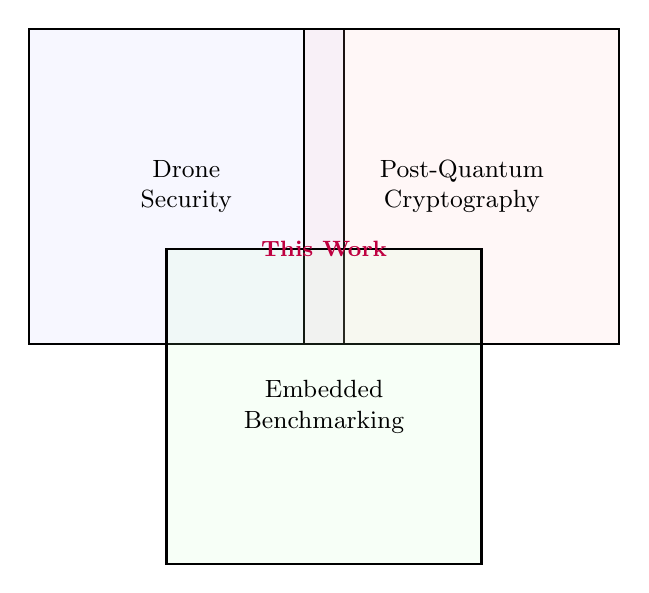
\begin{tikzpicture}[
  circle/.style={draw, thick, minimum size=4cm, fill opacity=0.1, text opacity=1, font=\small, align=center},
]
  \node[circle, fill=blue!30] (drone) at (0, 0) {Drone\\Security};
  \node[circle, fill=red!30] (pqc) at (3.5, 0) {Post-Quantum\\Cryptography};
  \node[circle, fill=green!30] (bench) at (1.75, -2.8) {Embedded\\Benchmarking};

  \node[font=\footnotesize\bfseries, text=purple] at (1.75, -0.8) {\textbf{This Work}};
\end{tikzpicture}
\caption{Research positioning: intersection of drone security,
post-quantum cryptography, and embedded benchmarking.}
\label{fig:rw-positioning}
\end{figure}

The novelty of our contribution is not in any single component---PQC
algorithms exist, drone security is studied, and ARM benchmarking has
been done---but in the \textbf{integration} of all three into a
single deployed, benchmarked, and documented system.

% ────────────────────────────────────────────────────────────────────────────
\section{Summary}
\label{sec:rw-summary}

\begin{itemize}
  \item Drone communication security research has grown rapidly, but
        \textbf{no published system} provides post-quantum encrypted
        MAVLink tunneling with comprehensive benchmarking.

  \item Post-quantum implementations exist for TLS, SSH, IPsec, and
        WireGuard, but all target desktop/server hardware.
        \textbf{No system targets real-time drone communication on ARM.}

  \item Lightweight cryptography (ASCON) and AES hardware acceleration
        are well-studied, but not in the context of a \textbf{multi-algorithm
        comparison framework} for drone security.

  \item MAVLink v2 signing is \textbf{inadequate}: no encryption, static keys,
        truncated signatures, no PQC.  Academic proposals (MAVSec,
        CryptoMAV, SecureLink) use classical cryptography only.

  \item PQC benchmarking exists at the \textbf{micro-benchmark} level
        (liboqs speed tests, PQM4) and the \textbf{protocol} level
        (PQ-TLS), but not at the \textbf{application} level with
        power measurement on embedded ARM hardware.

  \item Our system fills these gaps by providing a \textbf{transparent,
        algorithm-agile, post-quantum MAVLink tunnel} with 72~cipher
        suites, INA219 power measurement, and comprehensive timing
        metrics on Raspberry Pi hardware.
\end{itemize}
